%!TEX root = ../thesis.tex
%*******************************************************************************
%*********************************** Third Chapter *****************************
%*******************************************************************************

\chapter{Numerical Methods}  %Title of the Third Chapter

\ifpdf
    \graphicspath{{Chapter3/Figs/PDF/}{Chapter3/Figs/}}
\else
    \graphicspath{{Chapter3/Figs/}}
\fi

In this chapter, we are going to discuss the details of the numerical method used in \texttt{Gmunu} \cite{cheong2020gmunu,cheong2020gmunu_amr}.
In the fully-constrained scheme, the evolution of relativistic hydrodynamics in dynamical spacetime
consists of a set of coupled hyperbolic-elliptic system.
Firstly, we discuss the numerical method adopted for the hyperbolic system in \texttt{Gmunu},
including the high-resolution shock-capturing (HRSC) method and the finite volume method.
Then, we discuss the multigrid solver in \texttt{Gmunu},
which is used to solve the elliptic system.

%********************************** %First Section  **************************************
\section{High-resolution shock-capturing (HRSC) methods}
The high-resolution shock-capturing (HRSC) methods is a class of methods commonly used to
reproduce accurately the discontinuous features in the solution
with no spurious oscillation \cite{harten1997high}.
Note that the HRSC methods can be distinguished in \textit{finite-difference (conservative)} method
which evolves the \textit{pointwise values} of the solution,
and \textit{finit-volume (conservative)} method which evolves the \textit{cell average} of the solution.
Although the accuracy of finite-difference method can be extended to higher order easily,
it is extremely difficult to extend the method to general non-uniform grids \cite{merriman2003understanding}.
On the other hand,
the finite-volume methods are natural to conservative scheme as well as non-structured grid,
but the multidimensional reconstruction algorithm is complicated and computational expensive especially for higher-order method.\\
In this section,
we will first discuss the finite-volume conservative methods,
and then focus on the \textit{Godunov methods} which guarantee the upwind property of conservative non-linear equations \cite{van1999introduction}.

\subsection{Finite-volume conservative methods}\label{section3.1.1}
Given the conservative equation in orthogonal coordinate system $(x^1, x^2, x^3)$ in form
\begin{align}\label{eq:finite_vol_cons}
    \partial_t \mathbf{q} + \frac{1}{\sqrt{\hat{\gamma}}}\hat{\nabla}_i \left( \sqrt{\hat{\gamma}} \mathbf{f}^i \right)
    &= \mathbf{s} + \mathbf{s}_{geom},
\end{align}
where $\mathbf{q}$ are the conserved variables,
$\mathbf{f}^i$ are the flux terms, $\mathbf{s}$ are the source terms
and $\mathbf{s}_{geom}$ are the geometrical source term which is related to the 3-Christoffel symbol
$\hat{\Gamma}^i{}_{jk}$ of the reference metric $\hat{\gamma}_{ij}$.
We can then discretize equation (\ref{eq:finite_vol_cons}) on a computational domain divided into $N_1 \times N_2 \times N_3$ cells.
Each cells can be represented by a tuple of integers $(i,j,k)$ where $1 \leq i \leq N_1$, $1 \leq j \leq N_2$ and $1 \leq k \leq N_3$.
The cell bounds are given by
\begin{align}
    (x^1_{i-1/2}, &x^1_{i+1/2}), & (x^2_{j-1/2}, &x^2_{j+1/2}), & (x^3_{k-1/2}, &x^3_{k+1/2}).
\end{align}
Thus, the mesh cell spacing is
\begin{align}
    \Delta x^1_i &= x^1_{i+1/2} - x^1_{i-1/2}, & \Delta x^2_j &= x^2_{j+1/2}- x^2_{j-1/2}, & \Delta x^3_k &= x^3_{k+1/2} - x^3_{k-1/2},
\end{align}
and the cell centers are
\begin{align}
    x^1_i &= \frac{1}{2} \left(x^1_{i+1/2} + x^1_{i-1/2}\right), & x^2_j &= \frac{1}{2} \left( x^2_{j+1/2}- x^2_{j-1/2} \right), 
    & x^3_k &= \frac{1}{2} \left( x^3_{k+1/2} - x^3_{k-1/2} \right).
\end{align}
By integrating equation \ref{eq:finite_vol_cons} over cell volume and applying divergence theorem on the flux terms,
it becomes
\begin{align}
    \begin{split}
    \frac{d}{dt} \left\langle \mathbf{q} \right\rangle_{i,j,k} = - \frac{1}{\Delta V_{i,j,k}} \bigg\{ &\left[
    \left. \left( \left\langle \mathbf{f} \right\rangle^1 \Delta A^1 \right) \right|_{i+1/2,j,k} -
    \left. \left( \left\langle \mathbf{f} \right\rangle^1 \Delta A^1 \right) \right|_{i-1/2,j,k} \right] \\
    + &\left[
    \left. \left( \left\langle \mathbf{f} \right\rangle^2 \Delta A^2 \right) \right|_{i,j+1/2,k} -
    \left. \left( \left\langle \mathbf{f} \right\rangle^2 \Delta A^2 \right) \right|_{i,j-1/2,k} \right] \\
    + &\left[
    \left. \left( \left\langle \mathbf{f} \right\rangle^3 \Delta A^3 \right) \right|_{i,j,k+1/2} -
    \left. \left( \left\langle \mathbf{f} \right\rangle^3 \Delta A^3 \right) \right|_{i,j,k-1/2} \right] \bigg\} \\
    + &\left\langle \mathbf{s} \right\rangle_{i,j,k}
    + \left\langle \mathbf{s}_{geom} \right\rangle_{i,j,k}
    \end{split}
\end{align}
where the cell volume and the volume-average are defined as
\begin{align}
    \Delta V_{i,j,k} &\coloneqq \int_{cell} \sqrt{\hat{\gamma}} dx^1 dx^2 dx^3, &
    \left\langle \bullet \right\rangle &\coloneqq \frac{1}{\Delta V_{i,j,k}} \int_{cell} \bullet \sqrt{\hat{\gamma}} dx^1 dx^2 dx^3
\end{align},
while the cell surface and the surface-average are defined as
\begin{align}
    \Delta A^i &\coloneqq \int_{surface} \sqrt{\hat{\gamma}} dx^{j,j\neq i}, &
    \left\langle \bullet \right\rangle &\coloneqq \frac{1}{\Delta A^i} \int_{surface} \bullet \sqrt{\hat{\gamma}} dx^{j,j\neq i}.
\end{align}
Since the reference metric $\hat{\gamma}_{ij}$ is time-independent,
the cell volume, cell surface and the volume-averaged 3-Christoffel symbols
$\left\langle \hat{\Gamma}^i{}_{jk} \right\rangle$ in the geometrical source term
are determined once the coordinate is chosen.
We have included these quantities in Appendix \ref{A2}.

\subsection{Godunov methods}
\label{section3.1.2}
For simplicity, we consider one-dimensional hyperbolic conservation laws
\begin{align}\label{eq:conservation_law}
    \partial_t \mathbf{q}\left(x,t\right) + \partial_x \mathbf{f} \left[\mathbf{q}\left(x,t\right)\right] &= 0,
\end{align}
We apply the discretization on spatial domain into computing cell $I_j$ with size $\Delta x$
\begin{align}
    I_j &= \left[ x_{j-1/2},x_{j+1/2} \right], & \Delta x &= x_{j+1/2}-x_{j-1/2},
\end{align}
and time slices $\left[t^n, t^{n+1}\right]$.
Thus, equation (\ref{eq:conservation_law}) can be recasted into a \textit{conservative} scheme as
\begin{align}
    \left\langle\mathbf{q}\right\rangle^{n+1}_j &= \left\langle\mathbf{q}\right\rangle^n_j 
    + \frac{\Delta t}{\Delta x} \left( \left\langle\mathbf{f}\right\rangle_{j-1/2} - \left\langle\mathbf{f}\right\rangle_{j+1/2} \right),
\end{align}
where
\begin{align}
    \left\langle\mathbf{q}\right\rangle^{n}_j &\coloneqq \frac{1}{\Delta x} \int^{x_{j+1/2}}_{x_{j-1/2}} \mathbf{q} \left(x, t^n\right) dx
\end{align}
is the \textit{cell-average} and
\begin{align}
    \left\langle\mathbf{f}\right\rangle_{j\pm 1/2} &\coloneqq \frac{1}{\Delta t} \int^{t^{n+1}}_{t^n} \mathbf{f} \left[\mathbf{q}\left(x_{j\pm 1/2},t\right)\right] dt
\end{align}
is the \textit{numerical fluxes}.\\
In Godunov's original approach \cite{konstantinovich1959difference},
he considered a piecewise-constant distribution of data
\begin{align}
    \mathbf{q}(x, t^n) &=
    \begin{cases}
        \left\langle\mathbf{q}\right\rangle^{n}_j  &\text{if } x \leq x_{j+1/2}, \\
        \left\langle\mathbf{q}\right\rangle^{n}_{j+1}  &\text{if } x >x_{j+1/2},
    \end{cases}
\end{align}
and built a local Riemann problem 
$\mathcal{RP}\left(\left\langle \mathbf{q}\right\rangle_{L}, \left\langle \mathbf{q} \right\rangle_{R} \right)$
with left state $\left\langle \mathbf{q}\right\rangle_{L} = \left\langle\mathbf{q}\right\rangle^{n}_j$ and
right state $\left\langle \mathbf{q} \right\rangle_{R} = \left\langle\mathbf{q}\right\rangle^{n}_{j+1}$.
Therefore, the numerical fluxes
\begin{align}
    \left\langle\mathbf{f}\right\rangle_{j+ 1/2} &= 
    \frac{1}{\Delta t} \int^{t^{n+1}}_{t^n} \mathbf{f} \left[\mathbf{q}\left(x_{j+ 1/2},t\right)\right] dt
    = \mathcal{F}\left( \left\langle\mathbf{q}\right\rangle^{n}_j, \left\langle\mathbf{q}\right\rangle^{n}_{j+1} \right)
\end{align}
only depends on the two constant states $\left\langle\mathbf{q}\right\rangle^{n}_j$ and $\left\langle\mathbf{q}\right\rangle^{n}_{j+1}$.\\
Note that the Godunov method is a \textit{monotone method}.
Consider an explicit method of the type
\begin{align}
    \left\langle \mathbf{q}\right\rangle^{n+1}_j &=
    \mathcal{H} \left(\left\langle \mathbf{q}\right\rangle^n_j, \left\langle \mathbf{q}\right\rangle^n_{j\pm 1},
    \left\langle \mathbf{q}\right\rangle^n_{j\pm 2}, \dots,
    \left\langle \mathbf{q}\right\rangle^{n-m}_j,\left\langle \mathbf{q}\right\rangle^{n-m}_{j\pm 1},
    \left\langle \mathbf{q}\right\rangle^{n-m}_{j\pm 2}, \dots \right).
\end{align}
The method is \textit{monotone} if
\begin{align}
    \frac{\partial \mathcal{H}}{\partial \left\langle \mathbf{q}\right\rangle^n_j } &\geq 0
    \quad \forall \left\langle \mathbf{q}\right\rangle^n_j.
\end{align}
From this definition, we can further prove that given the data $\{ \left\langle \mathbf{q}\right\rangle^n_j \}$,
the solution $\{ \left\langle \mathbf{q}\right\rangle^{n+1}_j \}$ obtained by a monotone method is
\begin{align}
    \max_{j} \{ \left\langle \mathbf{q}\right\rangle^{n+1}_j \} &\leq \max_{j} \{\left\langle \mathbf{q}\right\rangle^n_j \}, &
    \min_{j} \{ \left\langle \mathbf{q}\right\rangle^{n+1}_j \} &\geq \min_{j} \{\left\langle \mathbf{q}\right\rangle^n_j \},
\end{align}
that is, no spurious new extrema introduced in the solution as time evolves.

\subsection{Reconstruction scheme}
The Godunov method introduced in the previous section is only first-order accurate in space and time
because of the piecewise-constant distribution of data.
In practice, the spatial accuracy can be higher than first-order 
if the left state $\left\langle \mathbf{q} \right\rangle_{L}$ 
and right state $\left\langle \mathbf{q} \right\rangle_{R}$ of the Riemann problem
at the cell interface $x_{j+1/2}$
are \textit{reconstructed} using a higher-order polynomial representation of $\mathbf{q}$
rather than $\left\langle \mathbf{q} \right\rangle^n_j$ and $\left\langle \mathbf{q} \right\rangle^n_{j+1}$.\\
One of the reconstruction techniques are the \textit{slope-limiter} methods 
which improve the piecewise-constant representation by providing a piecewise-linear reconstruction
of $\mathbf{q}^n(x)$ at each cell
\begin{align}
    \mathbf{q}^n_j (x) &= \left\langle \mathbf{q} \right\rangle^n_j + \mathbf{\sigma}^n_j \left(x-x_j \right) &
    \text{for } & x_{j-1/2} \leq x \leq x_{j+1/2},
\end{align}
where $\mathbf{\sigma}^n_j$ is the slope of the linear reconstruction.
Here, we list out several common slope-limiters
\paragraph{Minmod slope-limiter}
The \textit{minmod slope-limiter} \cite{ziegler2011semi,kolgan1972application,van1979towards}
is given by
\begin{align}
    \mathbf{\sigma}^n_j &\coloneqq \text{minmod}\left(
    \frac{\left\langle \mathbf{q} \right\rangle^n_j-\left\langle \mathbf{q} \right\rangle^n_{j-1}}{\Delta x},
    \frac{\left\langle \mathbf{q} \right\rangle^n_{j+1}-\left\langle \mathbf{q} \right\rangle^n_{j}}{\Delta x} \right),
\end{align}
where
\begin{align}
    \text{minmod}\left(\alpha, \beta \right) &\coloneqq
    \begin{cases}
        \alpha & \text{if } |\alpha|<|\beta| \text{ and } \alpha\beta>0, \\
        \beta & \text{if } |\alpha|>|\beta| \text{ and } \alpha\beta>0, \\
        0 & \text{if } \alpha\beta \leq 0,
    \end{cases}\\
    &\coloneqq \frac{1}{2}\left[ \text{sgn}{\alpha} + \text{sgn}{\beta} \right] \min \left(|\alpha|,|\beta| \right).
\end{align}

\paragraph{Monotonized central-difference (MC) limiter}
The MC limiter \cite{van1974towards} is given by
\begin{align}
    \mathbf{\sigma}^n_j &\coloneqq \text{minmod}\left(
    \frac{\left\langle \mathbf{q} \right\rangle^n_{j+1}-\left\langle \mathbf{q} \right\rangle^n_{j-1}}{2 \Delta x},
    \frac{\left\langle \mathbf{q} \right\rangle^n_j-\left\langle \mathbf{q} \right\rangle^n_{j-1}}{\Delta x},
    \frac{\left\langle \mathbf{q} \right\rangle^n_{j+1}-\left\langle \mathbf{q} \right\rangle^n_{j}}{\Delta x} \right),
\end{align}
where
\begin{align}
    \text{minmod}\left(\alpha, \beta, \gamma \right) &\coloneqq
    \begin{cases}
        \min\left(\alpha, \beta, \gamma\right) & \text{if } \alpha,\beta,\gamma > 0, \\
        \max\left(\alpha, \beta, \gamma\right) & \text{if } \alpha,\beta,\gamma < 0, \\
        0 & \text{otherwise}.
    \end{cases}
\end{align}\\
Note that the methods mentioned above are \textit{total variation diminishing (TVD)}.
The total variation of a solution at time $t^n$ is defined as
\begin{align}
    \text{TV}\left( \left\langle \mathbf{q} \right\rangle^n \right) &\coloneqq 
    \sum_i \left| \left\langle \mathbf{q} \right\rangle^n_{j+1} - \left\langle \mathbf{q} \right\rangle^n_j \right|,
\end{align}
which measures the oscillations appeared in the solution.
A numerical method is called \textit{total variation diminishing (TVD)} if it satisfies
\begin{align}\label{eq:TVD}
    \text{TV}\left( \left\langle \mathbf{q} \right\rangle^{n+1} \right) \leq
    \text{TV}\left( \left\langle \mathbf{q} \right\rangle^n \right), \quad \forall \left\langle \mathbf{q} \right\rangle^n,
\end{align}
which shows that the oscillations of the solution in TVD method are reduced.\\
Here, we list out all the possible reconstruction schemes in \texttt{Gmunu} in Table \ref{tab:limiters}.
\begin{table}[h]
	\centering
	\caption{\label{tab:limiters}Reconstruction schemes available in \texttt{Gmunu}.}
	\begin{tabular}{ l | l | l | l | l }
		\multicolumn{1}{c|}{ Order of accuracy } & \multicolumn{1}{c|}{ 2nd } & \multicolumn{1}{c|}{ 3rd } & \multicolumn{1}{c|}{ 5th } & \multicolumn{1}{c}{ 7th }\\ \hline
		  & Minmod \cite{ziegler2011semi,kolgan1972application,van1979towards} 
          & PPM \cite{colella1984piecewise} & MP5 \cite{suresh1997accurate} & WENO7\\
		  & MC \cite{van1974towards} & Koren & WENO5 & MP-WENO7 \\
		  & Superbee \cite{roe1986characteristic} & Cada3 & WENO5-Z & EXENO7 \\
		  & Vanleer \cite{van1977towards} & WENO3 & WENO5-Z+ &  \\
		  & Albada & WENO3-YC-3 & WENO-NM-5 &  \\
		  & MC-beta &  & WENO-NM-Z &  \\
		  & Cada &  & WENO-NM-Z+ &  \\
		  & Venk &  &  &  \\
	\end{tabular}
\end{table}

\subsection{Approximate Riemann solver}
As discussed in section \ref{section3.1.2},
the Godunov method requires the solution of local \textit{Riemann problem }
$RP\left(\left\langle \mathbf{q} \right\rangle_{L}, \left\langle \mathbf{q} \right\rangle_{R} \right)$
at the cell interface $x_{j+1/2}$ involving the left state $\left\langle \mathbf{q} \right\rangle_{L}$
and right state $\left\langle \mathbf{q} \right\rangle_{R}$.
Although the exact solution of the Riemann problem is available in relativistic hydrodynamics,
it is computational costly in multidimensional case.
Therefore, an \textit{approximate Riemann solver} is used in \texttt{Gmunu}
which is computationally less expensive and yet very accurate in general.
Approximation Riemann solver can be divided into two types
\begin{enumerate}[label=(\roman*)]
    \item \textit{Complete Riemann solver} which contains all the characteristic fields of the exact solution, and
    \item \textit{Incomplete Riemann solver} which only contains a subset of them.
\end{enumerate}
In this section, we discuss some commonly used incomplete Riemann solver in \texttt{Gmunu}.
For a comprehensive introduction, we refer readers to \cite{toro2013riemann}.

\paragraph{The HLL solver}
This Riemann solver was proposed by Harten, Lax and van Leer \cite{harten1983upstream}, hence the name \textit{HLL Riemann solver}.
The solution is approximated by
\begin{align}
    \mathbf{q}(x,t) &= 
    \begin{cases}
        \mathbf{q}_L & \text{if } x/t < \lambda_L, \\
        \mathbf{q}_{HLL} & \text{if } \lambda_L \leq x/t \leq \lambda_R, \\
        \mathbf{q}_R & \text{if } x/t > \lambda_R,
    \end{cases}
\end{align}
where $\lambda_L \leq 0$ and $\lambda_R \geq 0$ are the minimum and maximum of the characteristic speeds respectively
\begin{align}
    \lambda_L &\coloneqq \min\left(0, \lambda_- \left(\mathbf{q}_L\right), \lambda_- \left(\mathbf{q}_R\right) \right), \\
    \lambda_L &\coloneqq \max\left(0, \lambda_+ \left(\mathbf{q}_L\right), \lambda_+ \left(\mathbf{q}_R\right) \right),
\end{align}
and $\lambda_{\pm}$ are given by the eigenvalues of the hydrodynamics equations.
The single constant state $\mathbf{q}_{HLL}$ is given by
\begin{align}
    \mathbf{q}_{HLL} &= \frac{\lambda_R \mathbf{q}_R - \lambda_L \mathbf{q}_L + \mathbf{f}_L - \mathbf{f}_R}{\lambda_R-\lambda_L}.
\end{align}
Thus, the numerical fluxes can be calculated as
\begin{align}
    \mathbf{f} &=
    \begin{cases}
        \mathbf{f}_L & \text{if } x/t < \lambda_L, \\
        \mathbf{f}_{HLL} & \text{if } \lambda_L \leq x/t \leq \lambda_R, \\
        \mathbf{f}_R & \text{if } x/t > \lambda_R,
    \end{cases}
\end{align}
where the HLL fluxes are
\begin{align}\label{eq:HLL_flux}
    \mathbf{f}_{HLL} &=
    \frac{\lambda_R \mathbf{f}_L - \lambda_L \mathbf{f}_R + \lambda_L \lambda_R \left(\mathbf{q}_R - \mathbf{q}_L\right)}{\lambda_R-\lambda_L}
\end{align}

\paragraph{The Rusanov solver}
The \textit{Rusanov approximate Riemann solver} \cite{rusanov1962calculation},
also known as the \textit{total variation diminishing Lax-Friedrichs (TVDLF) flux} \cite{shu1989efficient},
is a special case of the HLL Riemann solver where the condition $\lambda_R = -\lambda_L = \lambda$ is imposed.
As a result, the Rusanov flux can be reduced from equation (\ref{eq:HLL_flux}) as
\begin{align}
    \mathbf{f}_{Rusanov} &= \frac{1}{2}\left(\mathbf{f}_L + \mathbf{f}_R \right) - \frac{1}{2}\lambda \left(\mathbf{q}_R - \mathbf{q}_L \right),
\end{align}
where one can take the single speed $\lambda$ to be $\lambda = \max\left(|\lambda_L|,|\lambda_R| \right)$.


%********************************** %Second Section  *************************************
\section{Time discretization}
\subsection{Explicit Runge-Kutta method}
To perform the time integration,
one can expand time derivative using Taylor expansion
\begin{align}
    \partial_t \mathbf{q} &= \frac{1}{2 \Delta t} \left(\mathbf{q}^{n+1} - \mathbf{q}^{n-1} \right).
\end{align}
However, it is not a practical time integration scheme because
\begin{enumerate}[label=(\roman*)]
    \item Large amount of data for the previous time steps is need to be stored in higher-order scheme.
    \item Stability is not guaranteed.
\end{enumerate}
In contrast, in the Runge-Kutta (RK) methods,
we do not need to store large amount of data, 
and it enables stable time integration for higher-order-accurate scheme.
Consider a system of equations in form
\begin{align}
    \frac{d \mathbf{q}}{dt} &= \mathbf{F} \left(\mathbf{q},t \right),
\end{align}
where $\mathbf{F}$ denotes the right-hand side of the equation.
The general $m$-stage explicit Runge-Kutta method of the Shu-Osher form \cite{shu1988efficient} is 
\begin{align}
    \mathbf{q}^{(0)} &= \mathbf{q}^n \\
    \mathbf{q}^{(i)} &= \sum^{i-1}_{k=0} \left[ \alpha_{ik} \mathbf{q}^{(k)} 
    + \Delta t \beta_{ik} \mathbf{F}\left( \mathbf{q}^{(k)}, t^n + \gamma_k \Delta t \right) \irght],
    \quad i=1,2,\dots,m \\
    \mathbf{q}^{n+1} &= \mathbf{q}^{(m)},
\end{align}
where the coefficient $\alpha_{ik}, \beta_{ik}$ and $\gamma_k$ are chosen such that the order conditions are satisfied.

\subsubsection{Strong stability-preserving (explicit) Runge-Kutta methods}
The strong stability-preserving Runge-Kutta (SSPRK) methods \cite{shu1988total,shu1988efficient}
is special class of RK methods which maintains total variation diminishing property (\ref{eq:TVD})
in higher-order time integration scheme.
Due to its non-oscillatory property,
the SSPRK methods are desirable in problems with discontinuities and strong shocks \cite{hesthaven2007nodal}.\\
As mentioned in section \ref{section1.5.3},
the hyperbolic system in the FCF scheme becomes unconditionally unstable
if first-order or second-order explicit RK method is used.
As a result, we use fourth-order SSPRK scheme to evolve the FCF hyperbolic sector 
and the hydrodynamics equation in \texttt{Gmunu}.

\subsection{Courant-Friedrichs-Lewy conditions}
One necessary condition for stability is the \textit{Courant-Friedrichs-Lewy} (CFL) conditions \cite{courant1928partiellen}.
From a physical point of view,
the CFL condition ensures that the propagation speed of any physical perturbation
is always smaller than the numerical speed $\lamda_N$
\begin{align}
    |\lambda| \leq \lambda_N \coloneqq \frac{\Delta x}{\Delta t}.
\end{align}
Therefore, the time steps for the time integration can be obtained by
\begin{align}
    \Delta t = c_{CFL} \min_k \left(\frac{\Delta x}{|\lambda_k|} \right),
\end{align}
where $c_{CFL}\leq 1$ is a dimensionless constant
and $\lambda_k$ is the characteristic speed of the evolution system.

%********************************** %Third Section  *************************************
\section{Atmosphere treatment}
One of the challenge in astrophysical simulation is handle the interface between fluid and vacuum
where the density $\rho$, pressure $p$ and velocities $v^i$ vanish.
In this section, we outline the positivity preserving limiter \cite{hu2013positivity,cheong2020gmunu_amr} used in $\texttt{Gmunu}$
for atmosphere handling.

\subsection{Positivity preserving limiter}
We consider a discretized first-order Euler timestep
\begin{align}
    &\frac{u^{n+1}_i - u^n_i}{\Delta t} = \frac{1}{\delta V_i} 
    \left( f_{i-1/2} \Delta A_{i-1/2} - f_{i+1/2} \Delta A_{i+1/2} \right),\\
    &\Rightarrow u^{n+1}_i = \frac{1}{2}\left( u^{+}_i - u^-_i \right),
\end{align}
where
\begin{align}
    u^-_i &\coloneqq \left( u^n_i - 2\frac{\Delta t}{\Delta V_i} f_{i+1/2} \Delta A_{i+1/2} \right), \\
    u^+_i &\coloneqq \left( u^n_i + 2\frac{\Delta t}{\Delta V_i} f_{i-1/2} \Delta A_{i-1/2} \right),
\end{align}
To ensure the positivity of $u^+_i$ and $u^-_i$, we modify the flux as \cite{hu2013positivity}
\begin{align}
    f_{i+1/2} &= \theta f_{i+1/2}^{HO} + (1-\theta) f_{i+1/2}^{LO},
\end{align}
where $f_{i+1/2}^{HO}$ is the original high-order flux scheme
and $f_{i+1/2}^{LO}$ is the first order Lax-Friedrichs flux.
The parameter $\theta \in \left[0,1\right]$ is the maximum value such that
$u^+_i$ and $u^-_i$ are positive.
Since the Lax-Friedrichs scheme is positivity preserving,
we can always choose $\theta$ to preserve the positvity.
Note that once the positivity in one first-order Euler timestep is preserved,
the positivity is guaranteed for any strong-stability preserving Runge-Kutta (SSPRK) time integrator.\\
In \texttt{Gmunu}, we implemented the positivity preserving limiter in conserved density $D$
and energy density $\tau$ to preserve the positivity of density $\rho$ and pressure $p$.
For the multidimensional case, we apply the limiter with component-by-component approach.

%********************************** %Fourth Section  *************************************
\section{Multigrid Method for elliptic equations} %Section - 3.1 
\label{section3.1}

\subsection{Overview} %Section - 3.1.1
\label{section3.1.1}
The elliptic equations can be solved using \textit{iterative methods} such as
Jocabi method, Gauss-Seidel (GS) method and successive overrelaxation (SOR) \cite{young2014iterative}.
These methods are very effective in eliminating high-frequency or
oscillatory components of the error,
but less effective in reducing low-frequency or smooth components of the error
since the changes of error are only made with spatially locally correction \cite{briggs2000multigrid}.
This problem will become even more severe for higher resolution 
because the convergence rate behaves like $1-\mathcal{O}(h^2)$.
Since the smooth modes in a fine grid become oscillatory in a coarser grid,
one can move to a coarser grid to smooth out the low-frequency mode error and return back to the fine grids.
This is the key idea of the multigrid method.\\
In the multigrid method, the key ingredients are
\begin{enumerate}[label=(\roman*)]
    \item \textbf{Multigrid cycle scheme} tells the structure of the multigrid solver (see Figure \ref{fig:MG_cycles} for example).
    \item \textbf{Restriction} maps the values from the fine grid to the coarse grid.
    \item \textbf{Prolongation} maps the values from the coarse grid to the fine grid.
    \item \textbf{Smoother} to smooth out the error at different levels.
    \item \textbf{Direct solver} to solve the equation at the coarsest level.
\end{enumerate}
\begin{figure}[h!]
	\centering
	\begin{subfigure}{0.3\columnwidth}
		\centering
        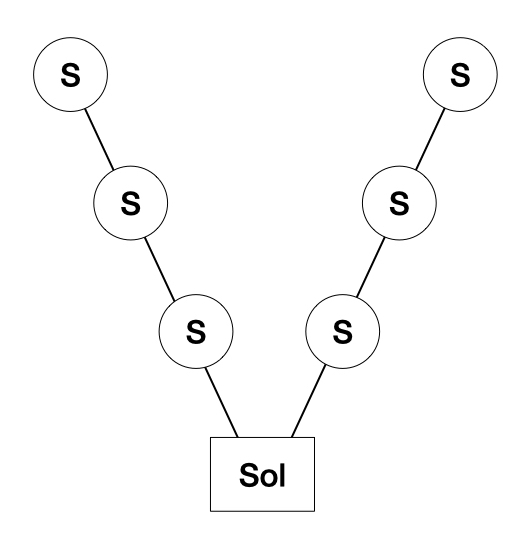
\includegraphics[width=\columnwidth]{MG_Vcycle.jpeg}
		\caption{V-cycle}
	\end{subfigure}
	%\hfill
	\begin{subfigure}{0.6\columnwidth}
		\centering
        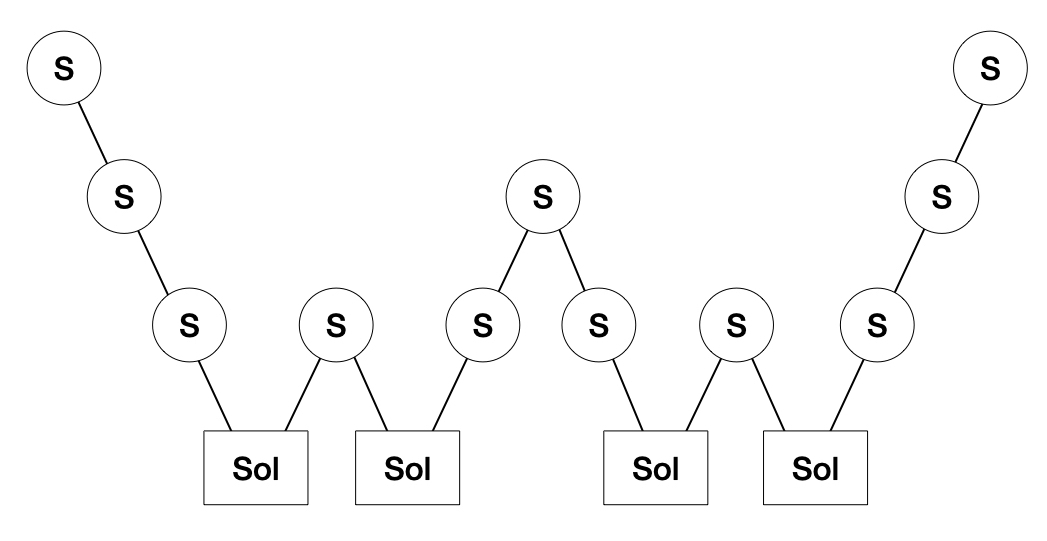
\includegraphics[width=\columnwidth]{MG_Wcycle.jpeg}
        \caption{W-cycle}
	\end{subfigure}

	\begin{subfigure}{0.45\columnwidth}
		\centering
        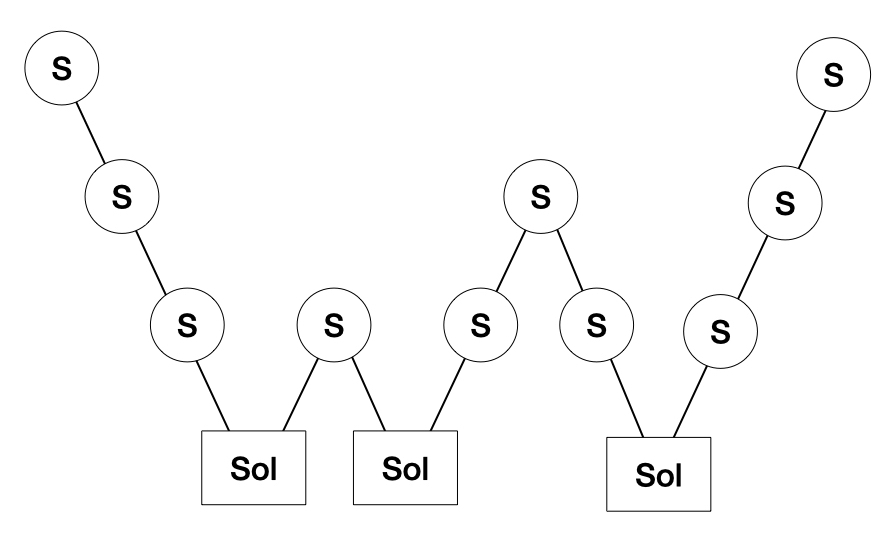
\includegraphics[width=\columnwidth]{MG_Fcycle.jpeg}
        \caption{F-cycle}
	\end{subfigure}
	\begin{subfigure}{0.45\columnwidth}
		\centering
        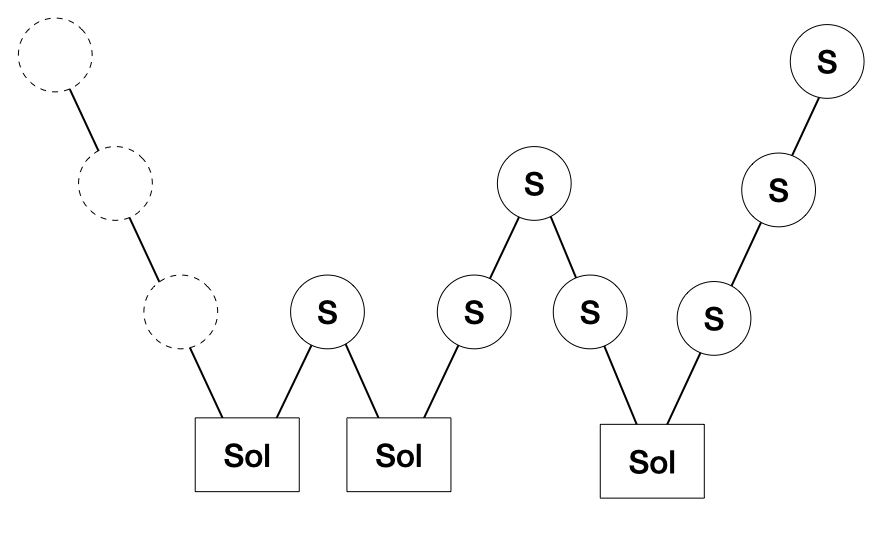
\includegraphics[width=\columnwidth]{MG_FMG.jpeg}
        \caption{Full multigrid (FMG) cycle}
	\end{subfigure}

	\begin{subfigure}{0.2\columnwidth}
		\centering
        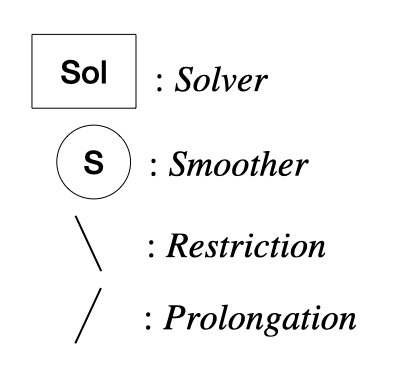
\includegraphics[width=\columnwidth]{MG_note.jpeg}
	\end{subfigure}

	\caption[Four different types of four-level cycles in multigrid methods.]{
		``S'' denotes smoothing. ``Sol'' denotes direct solver.
		Descending line $\setminus$ denotes restriction and ascending line / denotes prolongation.
	}
	\label{fig:MG_cycles}
\end{figure}

For more comprehensive discussion of multigrid method,
we refer the readers to \cite{briggs2000multigrid,trottenberg2000multigrid,young2014iterative,brandt2011multigrid}.

\subsection{Cell-centered discretization and operator} %Section - 3.1.2
\label{section3.1.2}
Given a non-linear elliptic equation 
\begin{align}
    \mathcal{L}\left(u\right) = f,
\end{align}
with elliptic operator $\mathcal{L}$, solution $u$ and source term $f$,
it can be discretized as
\begin{align}
    \mathcal{L}_h \left(u_h \right) = f_h,
\end{align}
where $\mathcal{L}_h$ is the discretized operator with resolution $h$,
$u_h$ and $f_h$ are solution and source term defined at the cell-centers.

\subsubsection{Laplacian operator}
The Laplacian operator is one of the elliptic operators that commonly used in \texttt{Gmunu},
including the constraint \cref{eq:XCFC_psi,eq:XCFC_alp} in XCFC scheme 
and the algebraic constraint \cref{eq:FCF_g_trace} in the FCF scheme.
It is discretized with a standard 5/7-point (in 2D/3D) second-order accurate discretization.
The details of the discretization in different geometry is shown in Appendix \ref{A1}.

\subsubsection{Mixed derivatives}
In the elliptic sector of the FCF scheme (\cref{eq:FCF_X,eq:FCF_psi,eq:FCF_alp,eq:FCF_beta})
and the vector elliptic equations in the XCFC scheme (\cref{eq:XCFC_X,eq:XCFC_beta}),
the elliptic operators contain mixed derivative terms $\frac{\partial^2 u}{\partial x \partial y}$.
We use second-order accuracy discretization as follows
\begin{align}
    \left(\frac{\partial^2 u}{\partial x \partial y} \right)_{i,j,k} &=
    \frac{u_{i+1,j+1,k} - u_{i-1,j+1,k} - u_{i+1,j-1,k} + u_{i-1,j-1,k}}{4 \Delta x \Delta y}
\end{align}

\subsubsection{Convection-diffusion equation}
In the momentum constraint (\cref{eq:FCF_X,eq:FCF_X_2}) of the FCF scheme,
the elliptic operator contains a convective term $\Delta^i{}_{kl}\left( L X \right)^{kl}$
which has a similar form as the following
\begin{align}\label{eq:convection_diff}
    \frac{\partial^2 u}{\partial x^2} + a \frac{\partial u}{\partial x} = 0.
\end{align}
While the Laplacian operator in equation (\ref{eq:convection_diff}) is discretized using standard 5/7-point approximation,
the convection term needs to be discretized using upwind method \cite{trottenberg2000multigrid}.
In \texttt{Gmunu}, we adopts second-order accuracy lopsided spatial finite difference as
\begin{align}
    \left(\frac{\partial u}{\partial x} \right)_i &= \frac{1}{2 \Delta x}
    \begin{cases}
        3 u_i - 4 u_{i-1} + u_{i-2} &\quad a \leq 0,\\
        -3 u_i + 4 u_{i+1} - u_{i+2} &\quad a \geq 0.
    \end{cases}
\end{align}

\subsection{Smoothers and solvers} %Section - 3.1.3
\label{section3.1.3}
Another essential element in multigrid method is the smoothers and direct solvers.
In \texttt{Gmunu}, we implemented the point-wise \textit{Newton Gauss-Seidel} smoothers \cite{press1996numerical}
\begin{align}
    u^{new}_{i,j,k} = u^{old}_{i,j,k} - \Bigg(\mathcal{L}\left(u^{old}_{i,j,k}\right) - f_{i,j,k} \Bigg)
    \left/ \left( \left. \frac{\partial \mathcal{L}}{\partial u_{i,j,k}}\right|_{u=u^{old}_{i,j,k}}\right)\right. ,
\end{align}
where the components of the new approximation are used as soon as they are computed.
Note that if $mathcal{L}$ is linear in $u$,
the Newton Gauss-Seidel method reduces to the standard Gauss-Seidel method.\\
There are two order of sweeping through the components $u_{i,j,k}$ implemented in \texttt{Gmunu}.
\begin{enumerate}
    \item \textit{Standard Gauss-Seidel} which follows the linear order of the indexes $i,j,k,$ stored in computer's memory.
    \item \textit{Red-black Gauss-Seidel} which sweeps through all the even indexes first (i.e. $i+j+k$ is even) then the odd indexes.
\end{enumerate}

Although the convergence rate of the smoothers is lowered in 2D/3D spherical and 3D cylindrical coordinate due to the anisotropy \cite{trottenberg2000multigrid},
currently we still implemented the smoothers for all coordinate.
For simplicity,
we adopt the Newton Gauss-Seidel method for the direct solver.

\subsection{Transfer operators: restriction and prolongation} %Section - 3.1.4
\label{section3.1.4}
The transfer operators connect data at different level.
The \textit{restriction} operators map the values from the fine grid to the coarse grid,
while the \textit{prolongation} operators map the values from the coarse grid to the fine grid.
For prolongation,
we use linear interpolation based on the nearest neighbors \cite{teunissen2019geometric,zhang2016boxlib,teunissen2018afivo},
which can be described by the following:
\begin{align}
    u_{x+h/2,y+h/2} &= \frac{1}{4} \left(2 u_{x,y} + u_{x+h, y} + u_{x,y+h} \right) + \mathcal{O}\left(h^2 \right),\\
    u_{x-h/2,y+h/2} &= \frac{1}{4} \left(2 u_{x,y} + u_{x-h, y} + u_{x,y+h} \right) + \mathcal{O}\left(h^2 \right),
\end{align}
or in stencil notation
\begin{align*}
	\frac{1}{4} \left]\begin{array}{ccccc}
		\cdot  & 1 &   & 1 & \cdot	\\
		1 & 2 &   & 2 & 1	\\
		  &   & * &   &  	\\
		1 & 2 &   & 2 & 1	\\
		\cdot & 1 &   & 1 & \cdot
	\end{array}\right[^h_{2h},
\end{align*}
where the ``$*$'' denotes the location of the coarse grid
and the notation shows the weighting of the value which are the neighbours of the coarse grid node ``$*$''.
For restriction, the value of four (2D) or eight (3D) fine grid values is averaged to obtain a coarse grid value.

\subsection{The Full Approximation Scheme} %Section - 3.1.5
\label{section3.1.5}
To solve the non-linear elliptic equations,
we adopt the Full Approximation Scheme (FAS) \cite{brandt1977multi,brabazon2014nonlinear,press1996numerical,cheong2020gmunu,teunissen2019geometric}.
Here, we briefly outline the FAS algorithm.
we define the residual $r$
\begin{align}
    r \coloneqq f - \mathcal{L} \left(v \right),
\end{align}
where $f$ is the right-hand side of the equation, 
$\mathcal{L}$ is the elliptic operator
and $v$ is an approximation solution.
For the discretized equation with resolution $h$, we have
\begin{align}
    r_h = f_h - \mathcal{L}_h \left( v_h \right).
\end{align}
The current approximation $v_h$ is then restricted to coarse grid
$v_{2h} = \mathcal{R} \left( v_h \right)$ where $\mathcal{R}$ is the restriction operator.
A copy of $v^{old}_{2h} = v_{2h}$ is stored for later usage. 
The coarse-grid right-hand side is then update as
\begin{align}
    f_{2h} = \mathcal{R} \left(r_h \right) + \mathcal{L}_{2h} \left(v_{2h} \right).
\end{align}
Smoothing steps are then applied to the coarse grid.
In the prolongation steps,
the solution is updated with a correction from the coarse grid as
\begin{align}
    v_{h} = v_{h} + \mathcal{P} \left(v_{2h} - v^{old}_{2h} \right),
\end{align}
where $mathcal{P}$ is the prolongation operator.
In practise, this procedure will be repeated until the solution converges
(i.e. the $L_\infty$ norm of the residual is below chosen threshold value).\\
Since the current version of \texttt{Gmunu} is built upon the framework of \texttt{AMRVAC 2.0} \cite{xia2018mpi,keppens2021mpi},
it is natural use the open-source geometric multigrid library \texttt{octree-mg} \cite{teunissen2019geometric} 
which is MPI-parallelized, support quadtree/octree AMR grids,
and provide periodic, Dirichlet, and Neumann boundary conditions.
Nonetheless, the library only supports 2D/3D Cartesian coordinate and 2D cylindrical coordinate.
We extended it to support multidimensional spherical and cylindrical coordinates as well as the Robin boundary condition.
In addition, only a single layer of ghost cell without diagonal cell is used in \texttt{octree-mg}.
In order to calculate the mixed derivatives and solve the convection-diffusion problems,
we extend the library to support multiple layers of ghost cells with diagonal cells,
which also allow us to explore higher-order scheme in the future.

